
% this file is called up by thesis.tex
% content in this file will be fed into the main document

%: ----------------------- introduction file header -----------------------
\chapter{Introduction}

% the code below specifies where the figures are stored
\graphicspath{{./1-introduction/figures/}}

% ----------------------------------------------------------------------
%: ----------------------- introduction content ----------------------- 
% ----------------------------------------------------------------------



%: ----------------------- HELP: latex document organisation
% the commands below help you to subdivide and organise your thesis
%    \chapter{}       = level 1, top level
%    \section{}       = level 2
%    \subsection{}    = level 3
%    \subsubsection{} = level 4
% note that everything after the percentage sign is hidden from output

The KM3NeT or the Cubic Kilometer Neutrino Telescope is currently being
constructed at the bottom of the Mediterranean Sea. The goal of this telescope
is two fold: first is to study high energy neutrinos originating from celestial
events such as birth of a neutrino star, supernovae, etc. and second, to study
the properties of the neutrino particles produced in the Earth's atmosphere
\cite{adrian2016letter}. The first goal will be realized with the KM3NeT/ARCA
(Astroparticle Research with Cosmics in the Abyss) telescope and the second
with KM3NeT/ORCA (Oscillation Research with Cosmics in the Abyss)
\cite{adrian2016letter}. In this paper, we talk exclusively about KM3NeT/ARCA.

\begin{figure}[h]
  \centering
  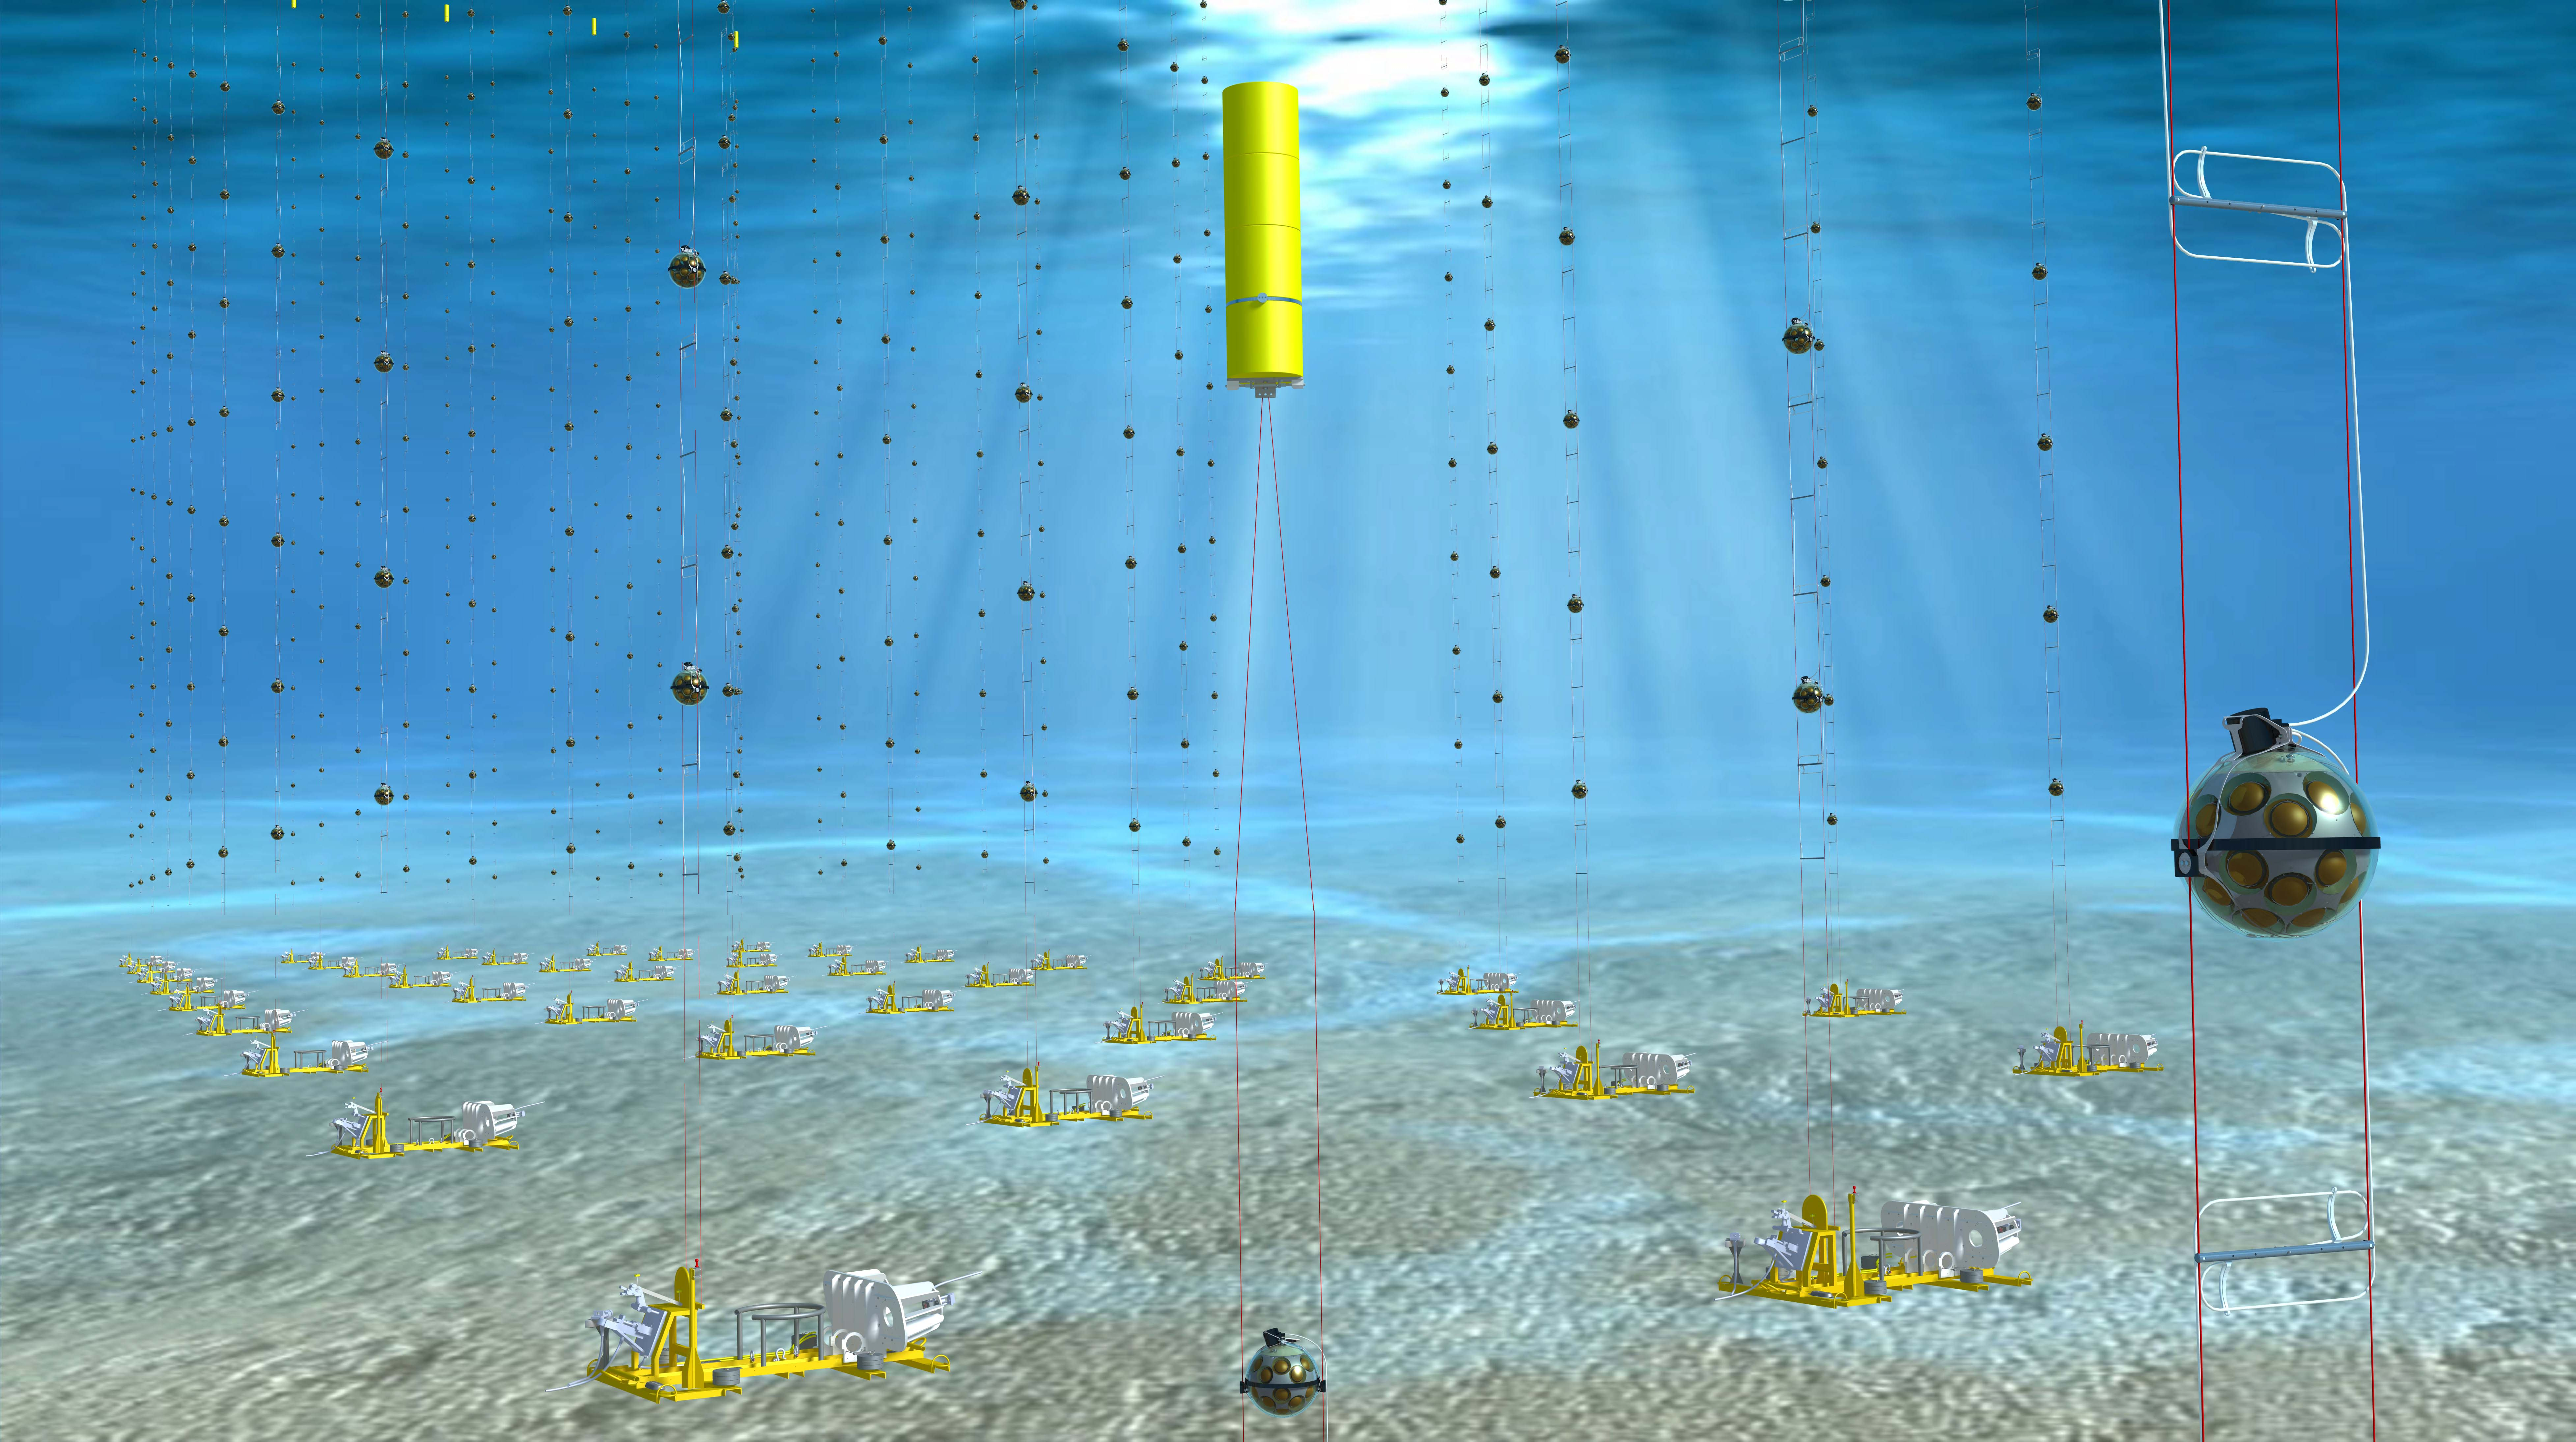
\includegraphics[width=\textwidth]{blocks.jpg}
  \caption{Artist's impression of the ARCA detector \textit{source: https://www.km3net.org}}%
  \label{fig:blocks}
\end{figure}

The ARCA telescope comprises of two ``blocks'' with a total volume of
$1km^{3}$. Each block consists of 115 spherical detector units (referred to as
DOMs henceforth) and each DOM consists of 31 Photo Multiplier Tubes (PMTs) in
various spacial arrangement. Figure \ref{fig:blocks} shows an artist's
impression of ARCA, figure \ref{fig:doms} depicts a DOM along with the PMTs
inside it.

\begin{figure}[h]
  \centering
  \includegraphics[width=0.5\textwidth]{doms.png}
  \caption{An optical detector (DOM) \textit{source: https://www.km3net.org}}%
  \label{fig:doms}
\end{figure}

The PMTs are sensitive to light or photons, the analog signal for all hits
above a certain threshold are digitized. This datapoint consists of a timestamp
and the spatial orientation of the DOM (ie. x,y,z coordinates). The digital
signals from all PMTs are arranged in 100ms ``time slices'' and sent to the
on-shore facility for further processing \cite{aiello2019km3net}.

\section{Situation of Concern}

When the high energy neutrino particles interact with surrounding matter,
produce an electron and a photon, this phenomenon is known as the Cherenkov
Radiation or Cherenkov Light \cite{margiotta2014km3net}. This phenomenon is
utilized in the KM3NeT telescopes to detect high energy neutrinos ie. the
Cherenkov Light is detected by the PMTs. Unfortunately, there are several
sources of noise (in this case, the noise is other light sources),
bioluminescense and decay of Potassium 40 ($^{40}K$) and atmospheric Muons being
the primary sources \cite{post2019km3nnet}.

\subsection{State of the Art}\label{state-of-the-art}

Due to the high level of noise, data is generated at an extremely high rate of
25GB/sec \cite{adrian2016letter}. Due to this high data rate, it must be
filtered and selectively stored for further analysis. The state of the art for
this task are known as ``Event Trigger'' algorithms
\cite{adrian2016letter,aiello2019km3net}. The existing event trigger algorithms
namely \emph{L1} and \emph{L2} have limitations and can be improved upon
\cite{karas2019data}.

There is a tradeoff between performance and quality of the event trigger
algorithms to be realized here. The state of the art \emph{L1} and \emph{L2}
algorithms are very performant with the ability to filter data in real time
however their quality of filtration can be improved. Thus new event trigger
algorithms must consider this trade off.

Efforts have already been made to improve the existing event trigger
algorithms. \cite{karas2019data} proposed and implemented a GPU powered
pipeline which utilizes correlation and graph community detection to identify
time slices that may contain neutrino hits whilst \cite{post2019km3nnet}
suggests an alternate using convolutional neural networks.

\subsection{User Requirements}\label{user-requirements}

The primary users of the ARCA are researchers who want to study high energy
particles from outer space. The stakeholders are all member institutes involved
in the project and by extension all scientists from these institutes who will
be working with the data collected.

The requirements of the primary users (and stakeholders) with respect to the
data acquisition pipeline are as follows: 1. The accuracy with which time
slices are filtered out has to be extremely high. Time slices which are deemed
important by event trigger algorithms are stored for further analysis and
research. Failure to store time slices containing important data can lead to
loss of important data and thus a poor quality of research. 2. The filtration
of noise must be highly accurate. The event trigger algorithms must be able to
eliminate majority of noise to prevent storage of unnecessary and potentially
useless data. 3. The state of the art event trigger algorithms are able to
process data in real time. The proposed alternative ideally should maintain or
improve upon it's predecessor's performance else provide a good trade off with
data quality.

\section{Research Question}

This report intends to improve upon the GPU pipeline proposed by
\cite{karas2019data}, specifically we wish to answer the following research
questions:

\begin{enumerate}
  \item[\textbf{RQ1}.] \textbf{Can the existing GPU pipeline be improved using neural networks (NNs)?}

    Specifically, improvement may be achieved by reducing the processing time
    of the pipeline or improving the accuracy of identifying important
    timeslices. In order to answer this research question, the following sub
    questions are formulated.

  \item[\textbf{RQ2.}] \textbf{Which NN will produce the best results when replaced with the \emph{Pattern Matrix}?}

    TODO add rational

  \item[\textbf{RQ3.}] \textbf{Which NN will produce the best results when replaced with the \emph{Graph Community Detection} algorithm?}

    TODO add rational
\end{enumerate}
